\subsection{KDE-based Reconstruction}
\label{sec:kde}

\textit{This section is a part of the PhD thesis of John Hardin, therefore, the coordinate systems and notations here are not the same compared to the previous text.}

\vspace{0.5cm}

In order to build a KDE based particle hypothesis PDF, the algorithm must quickly trace many photons from the charged particle path to the detection array.  This provides the $n$ $s_{i}$ in equation~\eqref{eq:kernel_form} in the next section {\em i.e.} it provides the many samples from a PDF required to estimate the PDF with Kernel Density Estimation (KDE).  FastDIRC leverages the symmetry of the bars to trace photons to the detector plane about 10000 times faster than \geant~\cite{Hardin:2016cvu}.

This tracing consists of a generation step, a step that traces through the bars, and a step which traces through the expansion volume.  We use the coordinate system shown in Fig.~\ref{pic:coord}.  The output of FastDIRC is a \deltall which is converted to a resolution as described in Appendix~\ref{app:resolution}.

\begin{figure}[!h]
  \begin{center}
    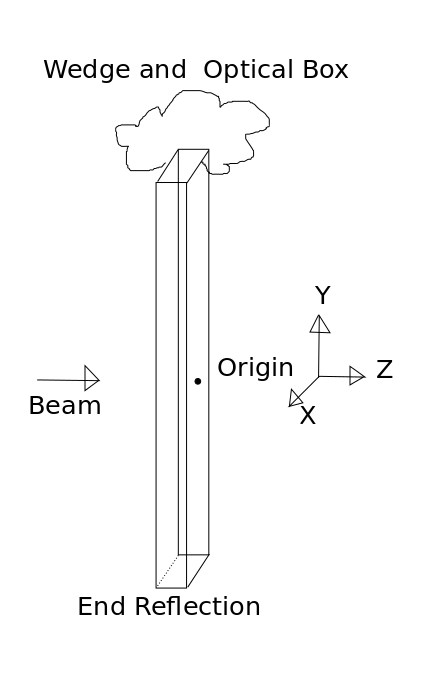
\includegraphics[width=.35\textwidth]{pics/billi.png}
    \caption{\label{pic:coord} 
      Coordinate system used when discussing the DIRC.  The sign of the $x$ direction is not relevant for reconstruction.}
  \end{center}
\end{figure}

\subsubsection*{Kernel Density Estimation}

One way to produce an estimate of the value of a probability density function at a point is to draw many points from that PDF and spread them with a kernel.  With enough points to resolve features, and a kernel sufficiently wide to provide smoothness, this results in a continuous estimate of the PDF which improves as the number of sampled point increases.  The algorithm presented in~\cite{Hardin:2016cvu} and implemented in FastDIRC generates a PDF in the 2 spatial coordinates (for the image plane) and time.

Let the set of $n$ points $\vec{s}$ be drawn from PDF $P$, then we can approximate $P$  as

\begin{equation}
P(x) \approx \sum_{i}^{n} K(x - s_{i}),
\label{eq:kernel_form}
\end{equation}
where $K$ is a decaying function of distance (often a gaussian), whose width is a decreasing function of the number of support points.  For the \gluex DIRC, the spatial and time resolution of the PMTs provide a natural scale around which to search for a kernel width.  A KDE allows for a continuous estimate of any PDF which can be sampled.

\subsubsection*{Tracing Through the Bars}
A significant hurdle to implementing a KDE estimator via traditional optics is the O(100) internal reflections that each photon undergoes as it propagates though the bar.  As O(600,000) KDE points are required for some hypotheses,\footnote{This number taken from the plateau of 5 GeV K-$\pi$ estimated for \gluex.  Lower energy particles can be well separated with less precise PDFs.} this results in a prohibitive number of multiplications for any large data set.  In order to overcome this, we take advantage of the fact that reflections can be mapped to drawing a straight line through a tiled plane.  Since rectangular prisms provide a simple tiling of the plane, it is only necessary to determine the ratio of the distances the particle travels in the $x-z$ plane to the distance it travels in $y$.  The distance in $y$ is known (this is just the distance to the end of the bar, or the distance through its image on the reflective end), making it easy to reconstruct the number of $x$ and the number of $y$ reflections by using integer division.  The parity of this integer tells us which direction the photon is now moving, while the remainder of the distance gives its position.  Tracing this way requires a constant, small amount of computation per photon to trace to the end of the bar, as opposed to the O(100) internal reflections that might otherwise be required.  See Fig.~\ref{fig:bounces_unfolding}.

\begin{figure}[!h]
\centering
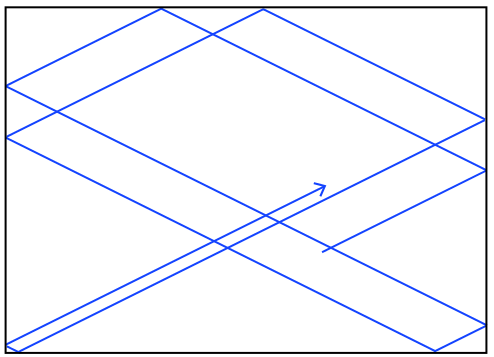
\includegraphics[width=0.45\textwidth]{pics/bouncesLarge.png}
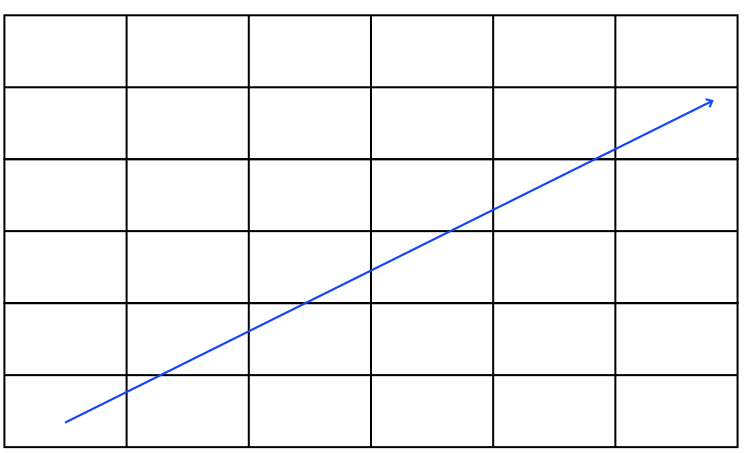
\includegraphics[width=0.54\textwidth]{pics/bouncesUnfolding.png}
\caption{Representation of the path of a photon looking down the $y$ axis of a DIRC bar (left).  Unfolding these bounces onto a grid for fast computation (right).}
\label{fig:bounces_unfolding}
\end{figure}


\subsubsection*{Generation}
While tracing is fast, it is still desirable to improve the speed of the algorithm.  One obvious way to do this is to only trace those photons which will produce a photoelectron {\em i.e.} apply the quantum efficiency before tracing the photon to the PMT plane.  As such, at generation, the Cherenkov wavelength PDF for the given $\beta$ of the particle is combined with the quantum efficiency PDF and the wavelength dependent index of fused silica to produce the PDF of the emission angles of photons.  
%See Fig.~\ref{fig:cerenkov_spectrum} for this distribution.  
This is implemented by a successive MC sampling of the Cherenkov wavelength and the quantum efficiency wavelength distributions.  
The wavelength is then used to compute the index of refraction, which is folded in with the particle speed to get a Cherenkov angle.  
The $\phi$ around the Cherenkov cone is sampled uniformly.

\subsubsection*{Optical Box Tracing}
At the end of the bars, the photons must then be traced to the readout plane.  It is desirable that this be done by dedicated code for speed.  The FastDIRC implementation allows an arbitrary class to perform this tracing.  As implemented for the \gluex optical box, the algorithm takes advantage of the fact that there are a finite number of sequences of reflection off of flat planes that a photon can take.  It then checks the case of each photon and simulates.  The output of this tracing is a point which contains the local $(x,y,t)$ coordinates of the PMT plane.

As this tracing is different for every DIRC geometry, the techniques for the \gluex geometry are discussed here.  In addition to the \gluex geometry, FastDIRC implements the geometry for \babar and the SuperB fDIRC prototype.

The \gluex geometry is a series of planar mirrors with a small number of possible paths for the light to take.  Each mirrored plane  is stored as 4 doubles: $a-d$ in the plane equation: $ax+by+cz=d$ or $\vec{N} \cdot \vec{x} = d$.  These numbers are used to simply and quickly compute plane intersection and reflection using the position and direction vector.  If we let $\vec{v}$ be the normalized direction the photon is moving, and we pick $d$ such that $\vec{N}$ is normalized, then the intersection and reflection of a plane is computed as follows:

\begin{equation}
t = -\frac{d + \vec{N} \cdot \vec{x}}{\vec{N} \cdot \vec{v}}
\end{equation}
\begin{equation}
\vec{x}_{intersect} = \vec{x} + t \cdot \vec{v}
\end{equation}
\begin{equation}
\vec{v}_{reflected} = \vec{v} + 2 \cdot (\vec{N} \cdot \vec{v}) \cdot \vec{N}.
\end{equation}
This computation can be done quickly, and small multiplication savings are had by computing both together.  Coordinates are provisionally intersected individually for testing between possible sequential reflections if the condition is otherwise too computationally intensive.  The computation of $t$ provides the distance which is used for timing information.  These techniques are used in the \gluex optical box simulation to decide which of the three segment mirrors to reflect off of and then perform the reflection.  The other mirrors in the box have their reflections performed by image projection---similar to how the propagation in the bars is done.  If the side mirrors (in the $y-z$ plane) are ignored, then any hit on the PMT plane that is outside the bounds can be reflected back after it touches the plane.  Similarly, by projecting to the image of the PMT plane in the large flat mirror rather than reflecting off of it, minor savings can be had.  See Fig.~\ref{fig:optical_box_optimize}.

\begin{figure}[!h]
\centering
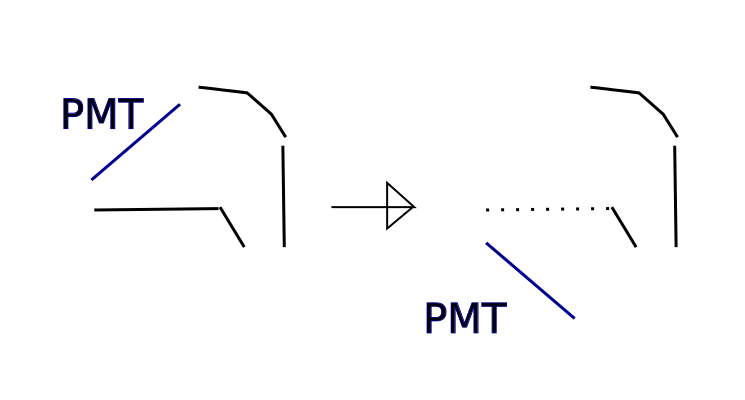
\includegraphics[width=0.7\textwidth]{pics/large_planar_pmt_project.png}
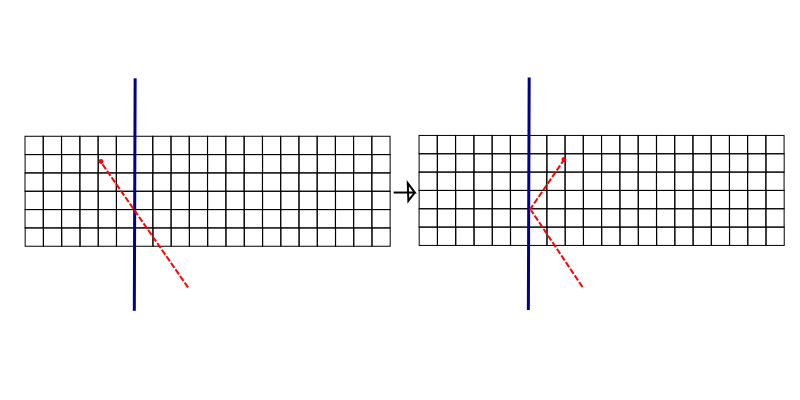
\includegraphics[width=0.7\textwidth]{pics/sidemirror_pmt_reflection.png}
\caption{Projection of the PMT plane in the large mirror (top).  The side mirrors are parallel to a coordinate plane, allowing even fewer multiplications (bottom).}
\label{fig:optical_box_optimize}
\end{figure}

The wedge is a special case; its sides are close enough together that multiple reflections off of them are common.  A strategy similar to the bars can be employed here, though FastDIRC currently implements this by looping in the $x$ direction using the method for the side mirror of the PMT plane, but iterated if the path reflects multiple times.  The wedge also has 2 distinct paths for light to propagate through it.  The light is likely to hit the 30\mydeg side (and totally internally reflect) before it exits the quartz and enters another optical medium (in the case of \gluex, this is water), but sometimes it changes optical media before it reflects off the 30\mydeg plane.  On the PMT plane, this creates a small structure slightly offset from the main pattern that looks somewhat like a mustache.  See Fig.~\ref{fig:wedge_paths}.

\begin{figure}[!h]
\centering
\includegraphics[width=0.48\textwidth]{pics/wedge_paths.pdf}
\caption{Possible light path through the wedge as projected into the $yz$ plane.  The vast majority of photons (dependent on incident particle kinematics) take the normal path with a few entering the water first and making a "Mustache".}
\label{fig:wedge_paths}
\end{figure}

For the implementation of the \gluex optical box, the $z$ intercept with particular planes is used to check where the photon will hit next.  By projecting the path and checking the $z$ bounds of the three planes in the three-segment mirror, the correct target can be obtained.  Similarly, the $z$ position when passing through the large planar mirror is used to reject photons which will not reach the plane (but would have due to the nature of FastDIRC treating the large mirror as nonexistent).

\begin{figure}[!h]
\centering
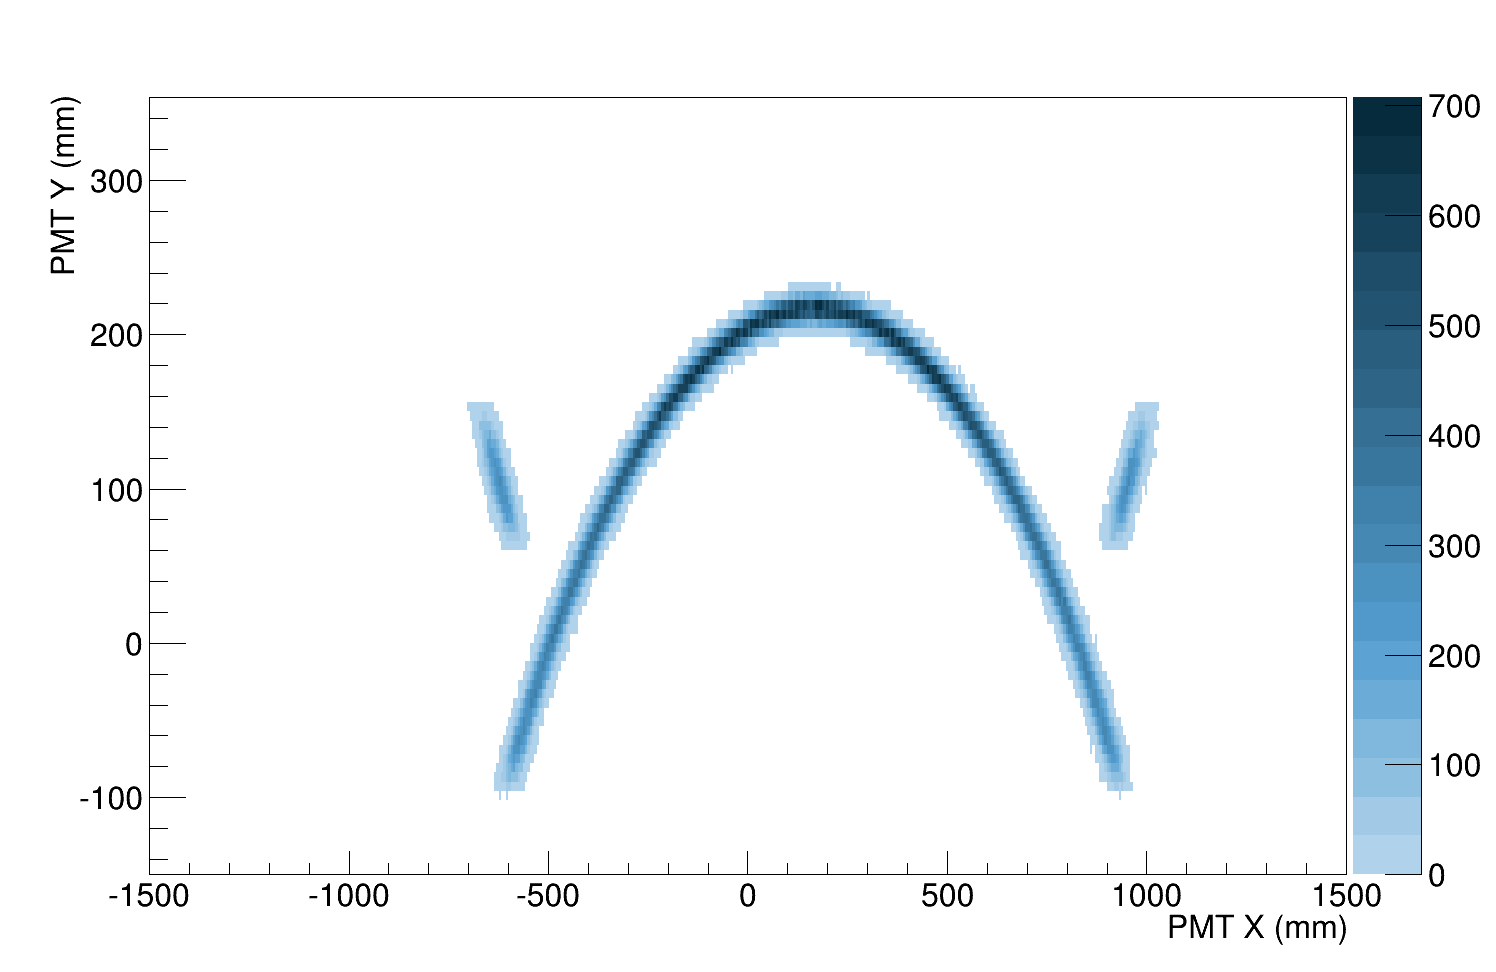
\includegraphics[width=0.49\textwidth]{pics/dist_cyl_perp_n147.png}
\includegraphics[width=0.49\textwidth]{pics/dist_cyl_perp_n133_edit.pdf}
%\put(-14,3.7){A.U.}
\caption{PDF of photons from a pion parallel to the $z$ axis and with a box that uses quartz as an optical medium and a cylindrical mirror (left).  PDF of the same pion with water as a medium (right).  Note that the ring is slightly wider, and the central mustache is visible.}
\end{figure}
\begin{figure}[!h]
\centering
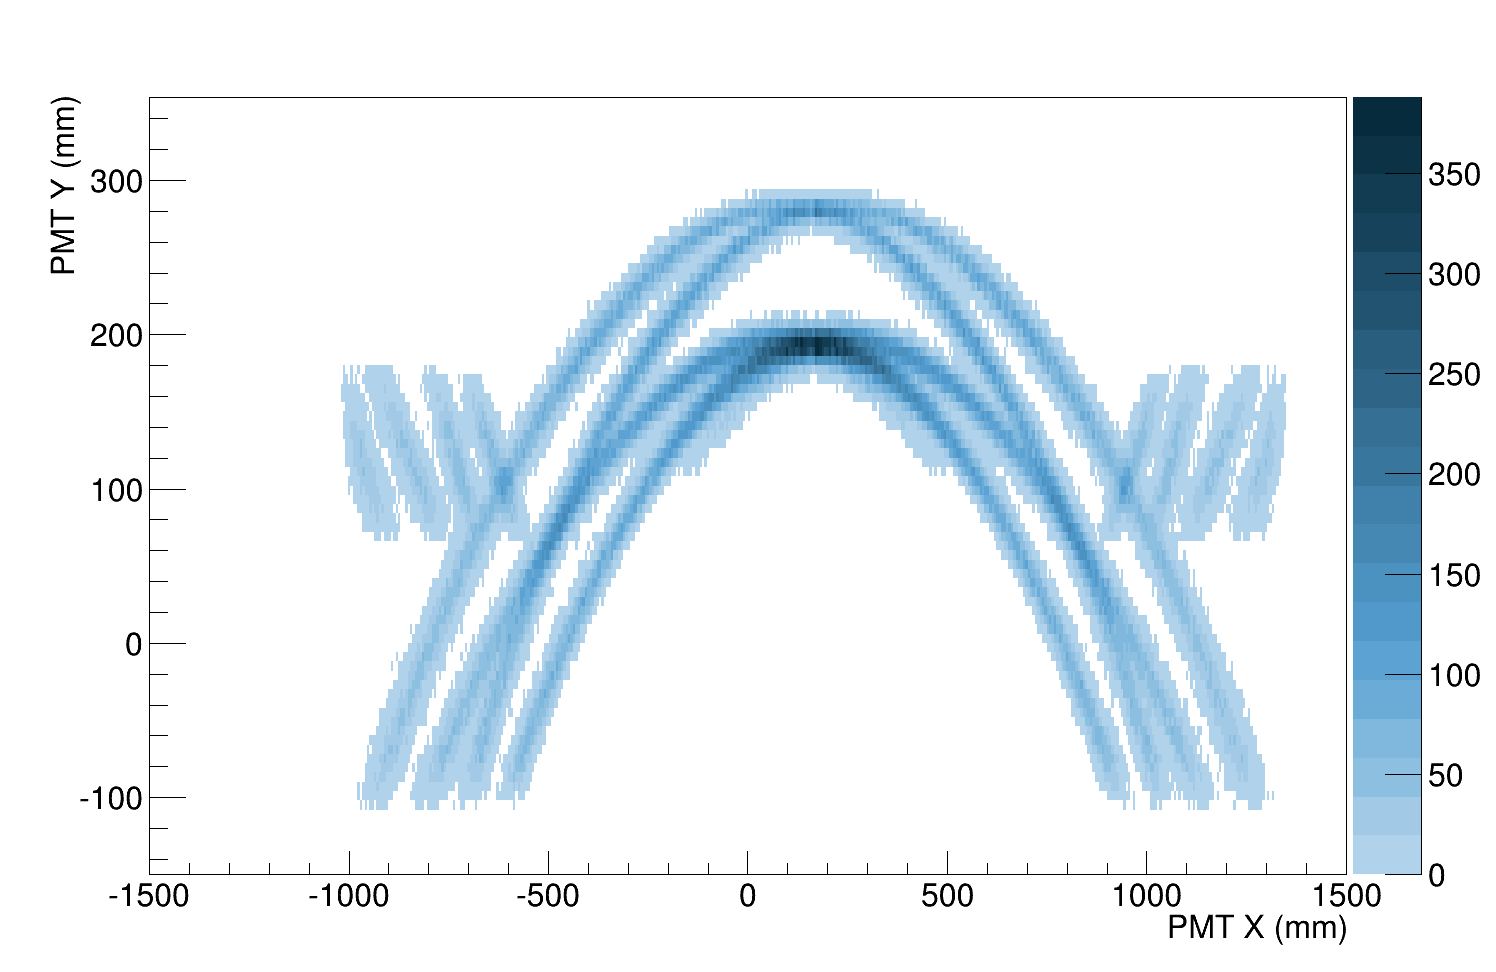
\includegraphics[width=0.49\textwidth]{pics/dist_cyl_440_n133.png}
\includegraphics[width=0.49\textwidth]{pics/dist_440_cannonical_pion_edit.pdf}
%\put(-14,3.7){A.U.}
\caption{PDF of photons from a pion at $\theta=4$ and $\phi=40$ degrees with a box that uses water as an optical medium on a cylindrical mirror (right).  PDF of photons from the same pion with a three segment mirror in the optical box (right).  Lines are drawn to help the eye connect up the image as it has been broken by reflecting off of non smooth planes.  The mustache is not visible in 2D, as it is under one of the major arcs, but these images are well separated in time.}
\label{fig:cyl_threeseg_recon}
\end{figure}

Shown in Fig.~\ref{fig:cyl_threeseg_recon} are the 4 different paths that the light takes out of the top of the bar along with the breaks where there are discontinuities in mirror angle.  In the cylindrical mirror image, the mustache that comes from the less often taken photon path is also shown.  It does not show up in the three segment mirror image because it is overlapping with one of the broken arcs.  What is not visible in the images is the timing of each of these hits.  The photons hit the plane over O(50 ns), and the PMTs are expected to have timing resolution of 1 ns or better.  While the arcs appear to overlap in 2 dimensions, they are well separated when timing information is added.

\subsubsection*{FastDIRC Implementation}

The FastDIRC code is hosted at~\cite{hardinGithub}.  There are a set of classes implementing tracking through a DIRC and providing an interface for various expansion volumes.  In its default run mode, FastDIRC generates each of a pion and kaon PDF once for a given particle kinematics and then simulates many particles with those kinematics and a normalized photon response.  The current driving program then stores this in a set of ROOT histograms, and a ROOT macro to convert these into an equivalent resolution is provided.  There are a variety of command line options to manipulate the geometry.

%\clearpage

\subsubsection*{Speed and Improvements}
The current algorithm can analyze approximately 3 particles/s on a laptop i7-3720QM 2.6GHz.  This is more than sufficient for design work, but is not sufficient to process large amounts of experimental data as a main algorithm.  Several ways to improve the speed are listed here.

Two methods that reduce the computation time of the lower level functions are faster trigonometric computation and better random sampling.  A profiling program reveals that trigonometry and random sampling are the function calls using the largest amount of CPU time.  The trigonometry can be improved by expanding some of the common calls in Taylor series.  The $\arccos$ call in the generation loop is only evaluated over a small range.  The mersenne twister algorithm used for random sampling is the other major CPU user.  Again, the photon generation uses multiple stages of rejection sampling to determine the wavelength.  Converting the function using inversion sampling would reduce the amount of random calls by more than 65\%.

Aside from low-level improvements, a progressive separation, which only simulates the number of points in the KDE that are required to separate the current image is also possible.  Momentum tested KDE filling would further provide performance gains: it has been observed that for well separated (low momentum) particles, the KDE requires significantly fewer photons before its performance begins to plateau, and in experimental data, many particles are at a momentum lower than the absolute required reach of the PID system.

One last major improvement would be to move to GPU-based computing.  GPUs are optimized for parallel ray tracing, which is exactly the task required to build the KDE.  Not all clusters have these resources available, but this method could take full advantage of those that do.

%\subsubsection{Middle line}

One possible extension of the current algorithm is to numerically calculate the central line through the pattern and use a spreading function around that.  Finding the central line, however, is nontrivial, as points along the curve do not correspond monotonically to the angle that they are emitted at around the Cherenkov cone.

Naively, one might expect that there is a simple correlation between progress along the 4 arcs and the $\phi$ around the Cherenkov cone.  By picking a central Cherenkov angle and removing the uncertainty from the $\theta$, the middle of the path can be traced.  As a function of this $\phi$, in fact, the image is essentially double valued.  See Fig.~\ref{fig:double_dirc_image}.

\begin{figure}[!h]
\centering
\includegraphics[width=0.7\textwidth]{pics/DoubleVals.pdf}
\caption{A single Cherenkov angle with sequential $\phi_{cone}$ values connected.}
\label{fig:double_dirc_image}
\end{figure}

Each half of the image is filled by the 2$\pi$ cycle around the Cherenkov cone.  To account for this, trace the image based only on photons having hit one of the two last $y-z$ sides of the bar {\em i.e.} only trace photons moving in the negative $x$ direction on exiting the bar.  This procedure results in the image in Fig.~\ref{fig:single_tracing}.

\begin{figure}[!h]
\centering
\includegraphics[width=0.7\textwidth]{pics/phi10k.pdf}
\caption{A single Cherenkov angle connecting $\phi_{cone}$ over $[0,2\pi]$ when the photons that bounce off one side plane are not traced.}
\label{fig:single_tracing}
\end{figure}

While the figure has removed the double valued nature, and does not have thickness from the Cherenkov angle spread, it still includes the {\em Kaleidoscope} effect.  The Kaleidoscope effect is the zig-zag pattern that the $\phi$ projection traces along the ring.  It comes from the fact that, when projected onto the grid shown for the bar optimization, the Cherenkov cone makes a parabola with a small part of the arc inside of each rectangle.  That arc corresponds to a finite interval in $\phi$ space and is continuously translated onto the PMT plane.  To get rid of the arcs making this substructure, we decrease the amount of $\phi$ domain they consume by making the bar arbitrarily thin (so that it almost looks like a plane).  While this increases the number of nominal bounces, our propagation time is independent of bounce number, so it has no effect on speed.  Once the photon reaches the top of this wafer, it is adjusted to that its $v_z$ is positive and it is sitting directly in the middle of the top of the bar.  This, combined with the selection for the last wall hit\footnote{As implemented, the last wall hit alternates between adjacent $\phi$, beacuse the last wall is not well defined in an infinitely thin wedge.} produces a smooth line through the middle of the image.  See Fig.~\ref{fig:single_tracing_line}.

\begin{figure}[!h]
\centering
\includegraphics[width=0.7\textwidth]{pics/line_overpoints_2d.pdf}
\caption{The line drawn with 10k $\phi$ points over the half of the pattern it corresponds to.  Again using the $\theta=4\eqdeg$, $\phi=40\eqdeg$ kinematics.}
\label{fig:single_tracing_line}
\end{figure}

The line traces the entire structure save for the mustache.  In this geometry, the mustache can only be produced by a photon close to $z=0$ when it exits the bar.  In the approximation of an infinitely thin bar, the photon is exiting at the middle of the bar.  This is visible in the $y$ versus Cherenkov $\phi$ plot.  This represents a small number of photons, and should minimally impact reconstruction, but it could be corrected by producing another ring in a future study.  The breakdown of the line's path in $x$, $y$, and $t$ appears in Fig.~\ref{fig:single_line_breakout}.

\begin{figure}[!htb]
\centering
\includegraphics[width=0.49\textwidth]{pics/line_overt_v_phi.pdf}
\includegraphics[width=0.49\textwidth]{pics/line_overx_v_phi.pdf}
\includegraphics[width=0.49\textwidth]{pics/line_overy_v_phi.pdf}
\caption{The time of intersection versus Cherenkov $\phi$ (left).  The $x$ location of intersection versus Cherenkov $\phi$ (right).  The $y$ location of intersection versus Cherenkov $\phi$ (bottom).}
\label{fig:single_line_breakout}
\end{figure}

One tested method of using this line to analyze a particle uses 10k initial points to make the line for both a pion and a kaon.  Then each of the experimental hits finds the closest point to it on this line and takes a weighted distance with spreads similar to the kernel of the original KDE.  After some minimal optimization of the parameters of this procedure, the separation returned is approximately 20\% worse than the full simulation with only 2\% as many support points required.  The analysis of possible algorithms leveraging the middle line was left at this point.  The main FastDIRC driver contains code to implement the line.

\clearpage

\subsubsection*{FastDIRC Performance}

FastDIRC as implemented provides for a basic LUT reconstruction implementation using the same information from the PMT plane.  This allows comparison of the two reconstruction methods on an equal footing.  To make the comparison more direct, the output of the LUT was translated to a resolution through the same ROC curve based method as the output of the KDE.  The resolution of FastDIRC over the kinematic region of the DIRC is shown in Fig.~\ref{fig:FastDIRC_performance}.  The performance of the LUT with and without a basic chromatic correction can be seen in Fig.~\ref{fig:lut_performance}.  The comparison of FastDIRC to a LUT is shown in Fig.~\ref{fig:FastDIRC_lut_comparison}.

\begin{figure}[!h]
\centering
\includegraphics[width=0.49\textwidth]{pics/lut_map_chrom.pdf}
\includegraphics[width=0.49\textwidth]{pics/lut_map_nochrom.pdf}
\caption{Resolution from LUT-based reconstruction using a chromatic correction (left).  Same without a chromatic correction (right).}
\label{fig:lut_performance}
\end{figure}

\begin{figure}[!h]
\centering
\includegraphics[width=0.7\textwidth]{pics/kde_map.pdf}
\caption{Resolution from FastDIRC created KDE PDFs.}
\label{fig:FastDIRC_performance}
\end{figure}

\begin{figure}[!h]
\centering
\includegraphics[width=0.7\textwidth]{pics/lut_v_kde_map.pdf}
\caption{Fractional improvement $\left(\frac{\sigma_{LUT}-\sigma_{FastDIRC}}{\sigma_{LUT}}\right)$ in Cherenkov angle resolution when moving from KDE to LUT.}
\label{fig:FastDIRC_lut_comparison}
\end{figure}

The curved zones of worse resolution in these figures correspond to charged particle kinematics which produce significantly overlapped rings.  While there are attempts to improve LUT based reconstruction by more efficiently using timing information, the KDE based reconstruction outperforms this LUT over the entire region, and shows the most improvement where the rings overlap the most.  Sample distributions for all kinematics can be found at~\cite{hardinWebDists}.

The $\approx 30\%$ performance increase is unfortunately still CPU intensive.  Simulating a KDE for each particle is still O(1000) slower than evaluating a LUT despite the O(10000) speedup in tracing particles through the bars.  This is sufficient for design work, but would not permit use as a dedicated reconstruction algorithm as implemented.  The possible improvements detailed above might drive this time down, and it is possible to use a hybrid reconstruction, {\em i.e.} only attempt a KDE based return for sufficiently ambiguous LUT responses.

\subsubsection*{Resolution Definitions}
\label{app:resolution}
The \deltall based KDE method used to do K--$\pi$ separation in this thesis does not return a Cherenkov angle for a given set of hits, but rather a log likelihood difference between particle hypotheses.  If we want to compare this performance using a more physical "resolution," we can obtain a log likelihood difference for many simulated kaons and for many simulated pions.  By plotting the pion veto efficiency versus the kaon identification efficiency for each possible value of a cut on this set of log likelihoods, we obtain a ROC curve.  The integral of this ROC curve gives us a measure of separation performance that can be compared to the performance of a detector which returned an angle spread by a gaussian.  By picking the spread of this gaussian such that the ROC curve of the ideal gaussian detector matches the simulated \deltall ROC curve, we obtain a "matching" resolution for the algorithm.  This matching resolution behaves broadly as expected:  It scales as ${n_{pe}^{-\frac{1}{2}}}$, where $n_{pe}$ is the number of photoelectrons and adds in quadrature with other errors in the system.

\begin{figure}[!h]
\centering
\includegraphics[width=0.49\textwidth]{pics/overlap_5_4_40.pdf}
\includegraphics[width=0.49\textwidth]{pics/roc_curve_overlay_5_4_40.pdf}
\caption{The \deltall difference for pions and kaons plotted against each other at 5~GeV, $\theta=4\eqdeg$, $\phi=40\eqdeg$ (left).  The ROC curve associated with those overlapping histograms (red) and the ROC curve of 2 gaussians with mean separated by the same angle (4.2 mrad) with $\sigma$=1.46 mrad (dotted blue) (right).}
\label{fig:roc_curve}
\end{figure}

%\subsubsection*{Single Photon Resolution}
The ROC curves match well in Fig~\ref{fig:roc_curve}, implying that the performance is close to gaussian.  This extracted resolution has the expected property of varying as ${n_{pe}^{-\frac{1}{2}}}$.  Given this scaling, it is convient to quote a single photon resolution, which is just $\sigma_{res}{n_{pe}^{\frac{1}{2}}}$.
